\documentclass{article}


\usepackage{authblk}
\usepackage{listings, chngcntr}
\usepackage{textcomp}
\usepackage{float}
\usepackage[T1]{fontenc}
\usepackage{indentfirst}
\usepackage{graphicx}
\usepackage{array}
\usepackage{caption} 
\usepackage{hyperref}
\usepackage{verbatim}
\usepackage{float}
\usepackage{subcaption}
\usepackage{gensymb}

\begin{document}

\title{Lock In}
\author[1]{Woojin Han}
\affil[1]{Seoul National University, Seoul 151-747, Korea}
\maketitle

\begin{abstract}
    In this experiment,
\end{abstract}

\section{Introduction}

\subsection{Lock In detection}
\label{intro: lock_in_detection}
\subsection{Data Analysis Module}
 While performing a Lock-In experiment, detected oscilloscope results can be returned in the form of \textbf{.csv} or \textbf{.png} files.
 However, there are too many time points in each \textbf{.csv} file, it is recommended to read the oscilloscope screen for each detection.
 Also, each experiment has various parameters controlled by each panel so the modification of each data takes complicated forms.
 Therefore, I build a clean module for a Lock-In experiment result analysis that can help the successor in two big ways.

 First, it supports \verb|lock_in_data| type and \verb|read_png()| method so that helps to read \textbf{.png} file fast.
 To run this module, we need a labeled Excel file that informs the parameters and the picture name.
 For example, let the preamplifier experiment of gain 2, input signal frequency of $50  [kHz]$ be saved by the file name "TEK000056.png".
 Then the labeled Excel file should contain a row 2, 50, and 56.
 And also the column of the picture name should be "name".
 We must modify the \verb|get_data_labels()|, which is the detected value of the oscilloscope \textbf{.png} for each experiment.
 I assumed that each experiment is placed in a different sheet of Excel file.
 
 \begin{verbatim}
reading 183 out of 701
Commit data: 1960
Commit data: 208
Commit data: 45.72
Commit data: -45.58
1_amplitude : 1960
2_amplitude : 208
12_phase : 45.72
21_phase : -45.58
{'gain': 10.0, 'frequency(kHz)': 200}
 \end{verbatim}
 

 By running \verb|main.py|, the example output above prints out.
 The module crops the exact position of the oscilloscope screenshots in \verb|./ERROR.PNG|, the only work to do is to read the number in the image.
 The commission of data is grouped simultaneously in \verb|lock_in_data| type and saved by \verb|datum. pkl|.
 The \verb|datum| is a dictionary that contains each experiment and data conveniently.
 For example, \verb|datum['preamplifier'][0]| is data collected in the preamplifier circuit the first time.

 Second, this module makes the plotting even more convenient.
 The Lock-In experiment needs to control some parameters and only plots a graph with selected parameters and results.
 Therefore, there must be a repeated structure of a plotting code scheme, which is very uncomfortable and crummy.
 In \verb|lock_in_data.py| header have the method of \verb|phys_plot()| which supports the faster way to plot a list of \verb|lock_in_data| type.
 For example, the code following plots the ratio of \verb|data. results[0]| and \verb|data. results[1]| in the function of signal frequency, only for the gain parameter set by 1.

 \begin{verbatim}
    fig = lock_in_data.phys_plot(
        datum[experiment],
        'frequency(kHz)',
        lambda x : x.results[0]/x.results[1], 
        {'gain': 1},
        x_label="frequency [kHz]",
        y_label= "Amplitude_ratio",
        fmt = 'ko'
        )    
 \end{verbatim}

 Every code and raw data is uploaded in \cite{github}, it is complete by itself so that only running \verb|main.py| will help the successor to use this module.
 For window system users must change the \verb|./| to \verb|.\\| to detour compatibility.

\section{Methods}
\label{methods: start}
Apparatus: Signal Processor (\cite{signal_processor}), oscilloscope, function generator, MG910 Hall ellement(\cite{hall_sensor})
The Lock-In module has been set up in the intermediate physics experiment laboratory, at Seoul National University.
The signal processor from Teach Spin is modular architecture with multiple circuits such as a preamplifier, and low pass amplifier.
I subtly improve the experimental method, especially the circuit modification, to specify the phase difference between the signal and reference input.
Every result of each experiment is in \ref{results: start} with the same subsection name.

\subsection{Preamplifier}
 The preamplifier circuit is not modified.
 Fig. \ref{fig: preamplifier_circuit}(a) shows the preamplifier circuit I used.
 Fig. \ref{fig: preamplifier_circuit}(b) is one of the raw data results while performing the circuit.

 \begin{figure}[ht]
  \centering
  \begin{subfigure}[b]{6cm}
      \centering
      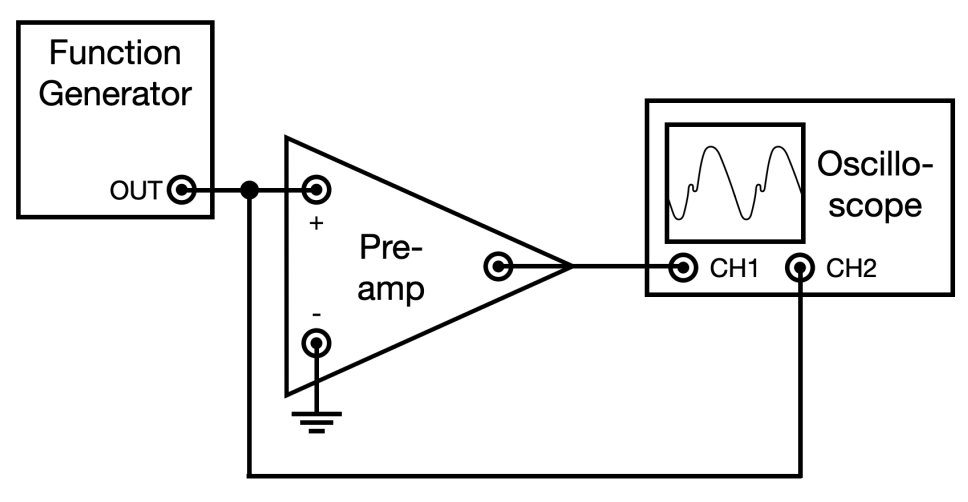
\includegraphics[width=6cm]{../results/preamplifier_circuit.png}
      \caption{}
  \end{subfigure}
  \hfill
  \begin{subfigure}[b]{6cm}
      \centering
      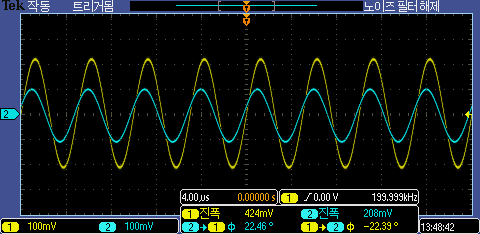
\includegraphics[width=6cm]{../raw_data/TEK00071.PNG}
      \caption{}
  \end{subfigure}
  \hfill
  \caption{Schematic diagram of (a) preamplifier circuit, adapted form  \cite{signal_processor}.
  (b)The oscilloscope screen capture of frequency 200 $kHz$ and gain$=2$.
  The blue line is the reference input and the yellow line is the signal output.}
  \label{fig: preamplifier_circuit}
\end{figure}
 I measured 57 different frequencies in each gain 1, 2, 5, 10, 20.
\subsection{Phase Shifter: Lagging phase detection}
The phase shifter provided in the signal processor is not uniformly performing, so the shifted phase is dependent on input signal frequency.
I define the word lagged phase as the difference between the real shifted phase and the displayed phase shift.
The manual suggests using the linear regression results of this measurement to complement the lagged phase, but as \ref{results: phase shifter} shows that the shifted phase amount is too big to cause errors.
Therefore I use three channels in the oscilloscope at the base of this circuit.
The first two of them are a reference and the phase-shifted signal just like this experiment circuit.
And the last one is set to the final signal of each experiment.
I have emphasized the modified circuit in each subsection.
\begin{figure}[ht]
    \centering
    \begin{subfigure}[b]{6cm}
        \centering
        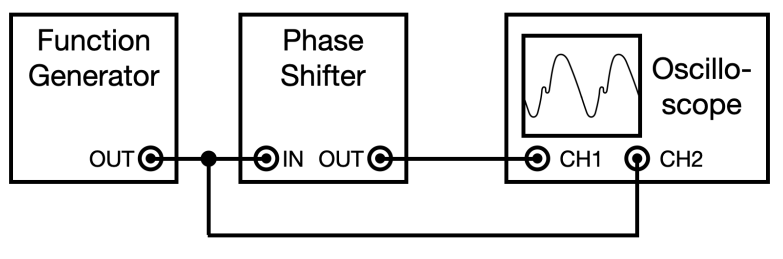
\includegraphics[width=6cm]{../results/phase_shifter_circuit.png}
        \caption{}
    \end{subfigure}
    \hfill
    \begin{subfigure}[b]{6cm}
        \centering
        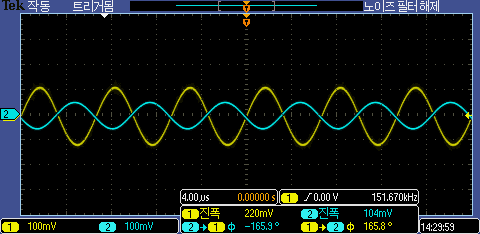
\includegraphics[width=6cm]{../raw_data/TEK00306.PNG}
        \caption{}
    \end{subfigure}
    \hfill
    \caption{Schematic diagram of (a) phase shifter circuit, adapted form  \cite{signal_processor}.
    (b)The oscilloscope screen capture of frequency 150 $Hz$ and $\pi/2$ phase shifted.
    The blue line is the reference input and the yellow line is the signal output.}
    \label{fig: phase_shifter_circuit}
  \end{figure}

 Fig. \ref{fig: phase_shifter_circuit}(b) shows the exact lagged phase in the module.
 The phase shifted amount displayed on the signal processor is $\pi/2$ but its real shifted phase is about $\pi$.
 I measured 17 different frequencies in each displayed phase shift value.

 \subsection{Lock In detection: DBM}
 The Lock-In detection is implemented by Double Balanced Mixer(DBM) explained at \ref{intro: lock_in_detection}.
 In this experiment, the DBM performance is checked.
 However, the lagged phase induced by the phase shifter and preamplifier huts the accurate measurement of the following experiments,
 I also display the phase-shifted input signal of the DBM module in the third channel of the oscilloscope.
 \begin{figure}[ht]
    \centering
    \begin{subfigure}[b]{6cm}
        \centering
        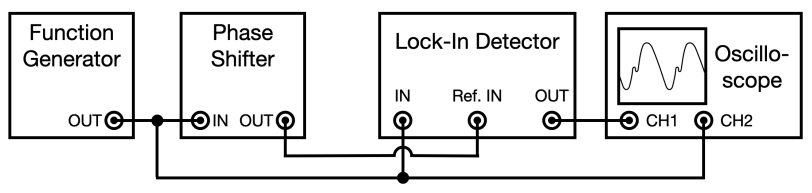
\includegraphics[width=6cm]{../results/DBM_circuit.png}
        \caption{}
    \end{subfigure}
    \hfill
    \begin{subfigure}[b]{6cm}
        \centering
        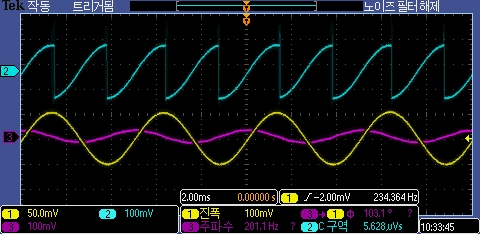
\includegraphics[width=6cm]{../raw_data/TEK00396.PNG}
        \caption{}
    \end{subfigure}
    \hfill
    \caption{Schematic diagram of (a) DBM circuit, adapted form  \cite{signal_processor}.
    (b)The oscilloscope screen capture of frequency 200 $Hz$ and $\pi/2$ phase shifted.
    The yellow line is the reference input and the purple line is the phase-shifted input.
    The blue line is the DBM output which performs well.
    }
    \label{fig: DBM_circuit}
  \end{figure}
 Fig. \ref{fig: DBM_circuit}(a) is the manual circuit arrangement, which has an inevitable error by the lagged phase.
 But by the subtle line connection, we can display the exact phase shit in the oscilloscope and can measure the real shift phase.
 So in the rest of the experiments, I modulate the phase difference by the measured value displayed in the oscilloscope.
 Fig. \ref{fig: DBM_circuit}(b) is the example results of the DBM experiment.
 It is definite to claim the phase difference between two input waves is $\pi/2$.
 But by the unavoidable error, the phase difference value fluctuates about $5\degree$, I read the median value while experimenting.
 I measured 21 different frequencies in each phase shift value of 0, $\pi/2$, $\pi$, and $3\pi/2$.

\subsection{Low-Pass Amplifier}
 The direct current offset is filtered by the low-pass amplifier.
 The amplifier has three parameters of $dB/oct$ and the time constant of the LC circuit.

 \begin{figure}[ht]
    \centering
    \begin{subfigure}[b]{6cm}
        \centering
        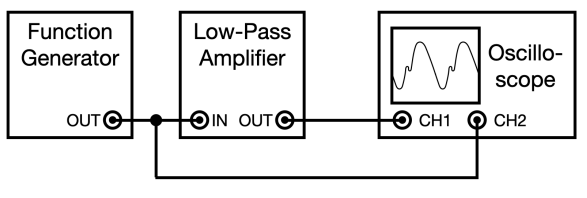
\includegraphics[width=6cm]{../results/low_pass_amplifier_circuit.png}
        \caption{}
    \end{subfigure}
    \hfill
    \begin{subfigure}[b]{6cm}
        \centering
        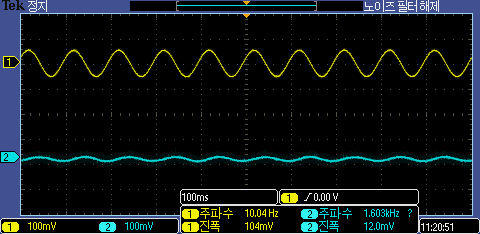
\includegraphics[width=6cm]{../raw_data/TEK00453.PNG}
        \caption{}
    \end{subfigure}
    \hfill
    \caption{Schematic diagram of (a) low pass amplifier circuit, adapted form  \cite{signal_processor}.
    (b)The oscilloscope screen capture of frequency 10 $Hz$ and $6 dB/oct$, the time constant of 0.1 s.
    The yellow line is the reference input and the blue line is the low-pass amplifier output which performs well.
    }
    \label{fig: low_pass_amplifier_circuit}
  \end{figure}

 Since it is applied to filter the high-frequency signals, in order of time constants, I have measured the signal for $0.1Hz$ to $50Hz$.
 The 10Hz result is even undetectable, as Fig. \ref{fig: low_pass_amplifier_circuit}(b) shows.
 Also widely broaden bandlike signal is observed, which is detailed in \ref{results: low pass filter}

 \subsection{Lock-In Amplifier: Noise detection}
 There are two steps in the noise detection experiment.
 The first is to check whether the noise provided by the signal processor is qualified by Fast Fourier Transform (FFT) included in the oscilloscope.
 The second is to form a Lock-In detection experiment to figure out a signal from the noise.
 \begin{figure}[ht]
    \centering
    \begin{subfigure}[b]{6cm}
        \centering
        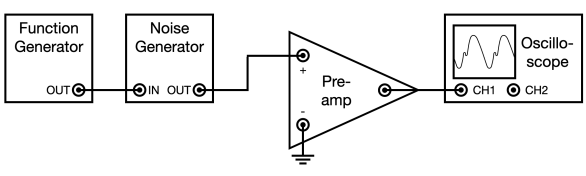
\includegraphics[width=6cm]{../results/noise_circuit.png}
        \caption{}
    \end{subfigure}
    \hfill
    \begin{subfigure}[b]{6cm}
        \centering
        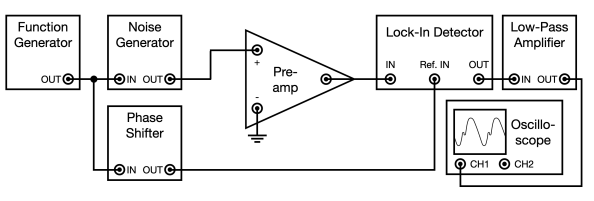
\includegraphics[width=6cm]{../results/noise_detection_circuit.png}
        \caption{}
    \end{subfigure}
    \hfill
    \caption{Schematic diagram of (a) noise generator and (b)the noise detection circuit, adapted form  \cite{signal_processor}.}
    \label{fig: noise detection}
  \end{figure}
 Fig. \ref{fig: noise detection}(a) shows the circuit of the first step.
 I put one plain channel to emphasize the noise signal with the unperturbed one.
 Fig. \ref{fig: noise detection}(b) represents the circuit of the second step.
 In this case, I plot a gain in the function of phase difference which must be measured precisely so that can give reliability to a regression.
 Therefore, I put two more channels in the oscilloscope, a reference and the noise signal each.
 The raw data of this experiment is plotted \ref{results: noise detection}.

\subsection{Lock-In detection: DC offset stability}
 To find a drift slope of a DC offset, the experiment is performed by the following circuit.
 Also, in this experiment the phase difference is fixed up to $\pi$, the circuit contains two more channels of reference and phase-shifted reference signal.
 \begin{figure}[ht]
    \centering
    \begin{subfigure}[b]{6cm}
        \centering
        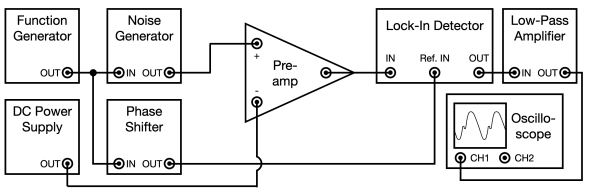
\includegraphics[width=6cm]{../results/DC_off_set_circuit.png}
        \caption{}
    \end{subfigure}
    \hfill
    \begin{subfigure}[b]{6cm}
        \centering
        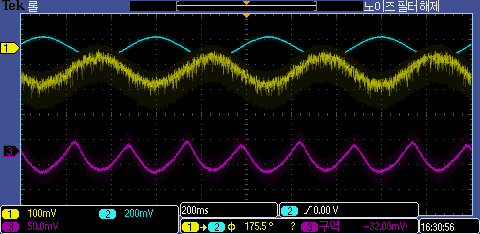
\includegraphics[width=6cm]{../raw_data/TEK00640.PNG}
        \caption{}
    \end{subfigure}
    \hfill
    \caption{Schematic diagram of (a) Lock-In DC offset stability measure circuit, adapted form  \cite{signal_processor}.
    (b)The oscilloscope screen capture of frequency 2 $Hz$ and $12 dB/oct$, the time constant of $0.03$ s the phase shifted value is $\pi$ the noise is added amount of $10^{-2}$.
    The blue line is the phase-shifted reference input and the yellow line is the noise-added signal.
    The purple line is the DBM Lock-In results.
    }
    \label{fig: DC_off_set_circuit}
  \end{figure}
 Fig. \ref{fig: DC_off_set_circuit}(a) is the circuit of the experiment.
 I used signal splitters in the Lock-In detector input and output to directly measure the phase difference between two inputs.
 Therefore, it can be very precisely controlled in this experiment, I have measured the gain from 25 different amounts of DC offset fixing phase difference in $\pi$.

 \subsection{Lock-In detection: Hall effect}
 The hall element signal is small so that the noise dominates the signal.
 Therefore, the frequency fixed Lock-In detection helps the signal distinguishable.
 The circuit is formed as the manual, but the phase difference is also directly measured as above experiments.
 \begin{figure}[ht]
    \centering
    \begin{subfigure}[b]{6cm}
        \centering
        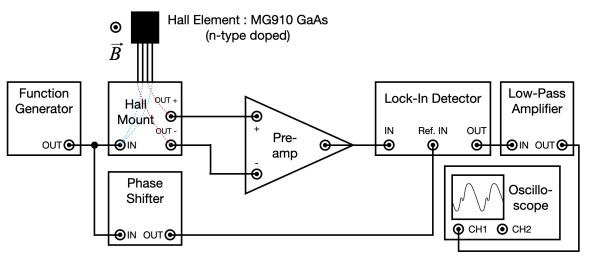
\includegraphics[width=6cm]{../results/hall_sensor_circuit.png}
        \caption{}
    \end{subfigure}
    \hfill
    \begin{subfigure}[b]{6cm}
        \centering
        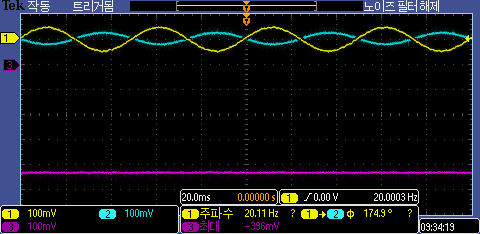
\includegraphics[width=6cm]{../raw_data/TEK00697.PNG}
        \caption{}
    \end{subfigure}
    \hfill
    \caption{Schematic diagram of (a) Hall element experiment circuit, adapted form  \cite{manual}.
    (b)The oscilloscope screen capture of frequency 20 $Hz$ and $12 dB/oct$, the time constant of $0.1$s, and the phase-shifted value is $\pi$.
    The yellow line is the phase-shifted reference input and the blue line is the Hall effect signal.
    The purple line is the Lock-In detected results.
    }
    \label{fig: hall_element_circuit}
  \end{figure}
 
 I measure the signal at 20 different distances at two different frequencies each.
 The Hall element sticks hard on the table, and the magnet distance is controlled by the wooden stick.
 Therefore, I can read the exact distance between the magnet and the Hall element in the measurement error of a few $mm$.

\section{Results and Discussion}
\label{results: start}
 Each subsection is labeled just as same with subsection from \ref{methods: start} respectively.
 The total codes and raw data of each parameter are uploaded to GitHub.
 (\cite{github}, \url{https://github.com/WoojinHan24/Lock_In})
 The specific file name of each plot is also obtained in Fig. \ref{fig: file_appendix}.

\begin{figure}[H]
    \begin{tabular}{ | m{8cm} | m{5cm}|  } 
      file name& details \\ 
      \hline
        \verb|preamplifier amp ratio freq plot(gainx).png| & preamplifier amplitude ratio - frequency plot in gain $x$
    \end{tabular}
    \caption{file appendix of \cite{github}}
    \label{fig: file_appendix}
\end{figure}

\subsection{Preamplifier}

\subsection{Phase Shifter: Lagging phase detection}
\label{results: phase shifter}

\subsection{DBM}

\subsection{Low Pass Filter}
\label{results: low pass filter}

\subsection{Lock-In Amplifier: Noise detection}
\label{results: noise detection}


\subsection{Lock-In detection: DC offset stability}



\subsection{Lock-In detection: Hall effect}



\section{Summary}

\cite{abcd}
\bibliography{lock_in_ref}
\bibliographystyle{plain}
\end{document}